%% 
%% Copyright 2019-2020 Elsevier Ltd
%% 
%% This file is part of the 'CAS Bundle'.
%% --------------------------------------
%% 
%% It may be distributed under the conditions of the LaTeX Project Public
%% License, either version 1.2 of this license or (at your option) any
%% later version.  The latest version of this license is in
%%    http://www.latex-project.org/lppl.txt
%% and version 1.2 or later is part of all distributions of LaTeX
%% version 1999/12/01 or later.
%% 
%% The list of all files belonging to the 'CAS Bundle' is
%% given in the file `manifest.txt'.
%% 
%% Template article for cas-dc documentclass for 
%% double column output.

%\documentclass[a4paper,fleqn,longmktitle]{cas-dc}
\documentclass[a4paper,fleqn]{cas-dc}

%\usepackage[authoryear,longnamesfirst]{natbib}
%\usepackage[authoryear]{natbib}
\usepackage[numbers]{natbib}

%%%Author definitions
\def\tsc#1{\csdef{#1}{\textsc{\lowercase{#1}}\xspace}}
\tsc{WGM}
\tsc{QE}
\tsc{EP}
\tsc{PMS}
\tsc{BEC}
\tsc{DE}
%%%

\begin{document}
\let\WriteBookmarks\relax
\def\floatpagepagefraction{1}
\def\textpagefraction{.001}
\shorttitle{Fingerprint reconstruction}
\shortauthors{Cristian Yesid Andrade Hernández et~al.}

\title [mode = title]{Fingerprint Reconstruction Using a Convolutional Generative Adversarial Model}                     

% AUTHOR 1
\author{Cristian Yesid Andrade Hernández}
\ead{cy.andrade@uniandes.edu.co}
\credit{Conceptualization of this study, Methodology, Software}

% AUTHOR 2
\author{Luis Felipe Giraldo Trujillo}
\ead{lf.giraldo404@uniandes.edu.co}
\credit{Thesis advisor}

\begin{abstract}
Biometric systems record fingerprints into digital platforms for allowing governments and organizations to have a structured and reliable way to identify people. In some cases, uncontrolled factors in both enrollment and verification processes make the biometric systems to obtain poor quality fingerprints records. Thus, performance of automatic identification decreases and the work of dactyloscopists becomes harder. This paper describes the implementation of a convolutional generative adversarial model that performs fingerprint image reconstruction in order to obtain clear ridge patterns using TensorFlow. Fingerprint enhancement boosts the correct extraction of fingerprint features called minutiae which are the center of matching and identification algorithms. A biometric open source framework called NBIS is used to measure the efectiveness of the model in terms of matching accuracy and image quality.
\end{abstract}

\begin{keywords}
fingerprint \sep enhancement \sep generative \sep adversarial \sep convolutional \sep neural \sep network
\end{keywords}

\maketitle

\section{Introduction}

Minutia based algorithms are the most widely used for fingerprint recognition. Minutiae are local ridge and valley characteristics of fingerprints such as endings and bifurcations \cite{HFPR}. Each minutia is determined by four values: pixel position in vertical axis, pixel position in horizontal axis, orientation and quality \cite{NBISUG}. Verification and identification algorithms compute a score based on the minutia of two fingerprints and if the score is above a certain threshold the fingerprints are determined to belong to the same person.

There are cases where quality of recorded fingerprints is poor due to factors like cut, wet, dry or burnt fingers, skin diseases, dirty scanning surfaces, incorrect pressure while scanning, among others. These factors remove real minutia or create false ones affecting the identification process. Fingerprint reconstruction allow matching algorithms to distinguish correctly between ridges and valleys, so real minutia is detected and identification accuracy improves.

Fingerprint enhancement can be treated as an image to image translation problem, so the solution proposed implements a generative adversarial convolutional neural network \cite{ITITAN}. It consists of a set of interconnected layers that receives an image as input, process it with convolutions and return the expected image as output. Parameters of the layer's filters are modified through an optimization process that minimize a cost function using a similarity measure and the adversarial training paradigm. 

Two main frameworks were used to develop the project: Tensorflow open source platform for building and training the model and NIST Biometric Image Software (NBIS) an open source biometric framework with core capabilities on fingerprint image processing developed by the National Institute of Standards and Technology (NIST) for the Federal Bureau of Investigation (FBI) and Department of Homeland Security (DHS) \cite{NBISWP}. Three NBIS modules were used in the project: \textit{mindtct} to extract minutiae in format \textit{xyt} from a fingerprint, \textit{bozorth3} to compute a similarity score between either a pair or a list of pairs of minutiae using the bozorth algorithm and \textit{nfiq} to return a quality measure of digital fingerprints.

The paper follows the next organization: source and preprocessing of training data is described in section \hyperref[sec:DP]{2}. Section \hyperref[sec:MA]{3} presents model architecture details. Training configuration is explained in section \hyperref[sec:MT]{4}. Section \hyperref[sec:R]{5} presents and analyses results. Finally, conclusion and future work are in sections \hyperref[sec:FW]{6} and \hyperref[sec:FW]{7} respectively.
     
\section{Data preprocessing}
\label{sec:DP}

Training data came from two sources: the first one is a private dataset of 19.859 fingerprints recorded during the enrollment process of citizen procedures. The second corresponds to 39.611 real fingerprints from LivDet dataset, a dataset built for a competition that rewards the best spoof detection model. Fig.~\ref{fig1} shows some examples of the datasets.

\begin{figure}[htbp]
\centerline{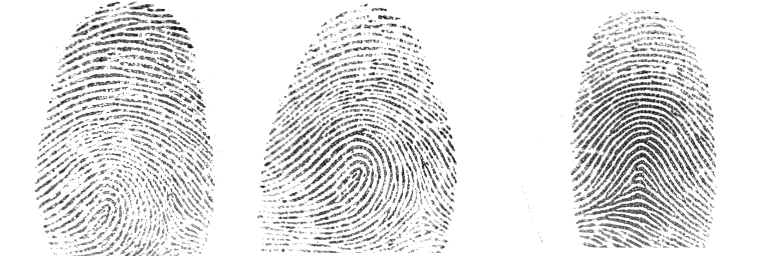
\includegraphics[scale=0.3]{figs/dataset_example.png}}
\caption{Example of images from source datasets}
\label{fig1}
\end{figure}

As data comes from different sources, the first step of preprocessing is to resize images into a resolution of 256x256. The next step is to build tuples, each one conformed by an image to enhance, and a target image. The image to enhance is obtained through an artificial deterioration process and the target image is the original image of the dataset. There are two types of deterioration. The first one consists in drawing noisy holes to simulate a skin disease, a burnt finger or other types of fingerprint modifications. It is achieved generating random white ellipses on images and summing a tiny gaussian noise as can be seen in Fig.~\ref{fig2}.

\begin{figure}[htbp]
\centerline{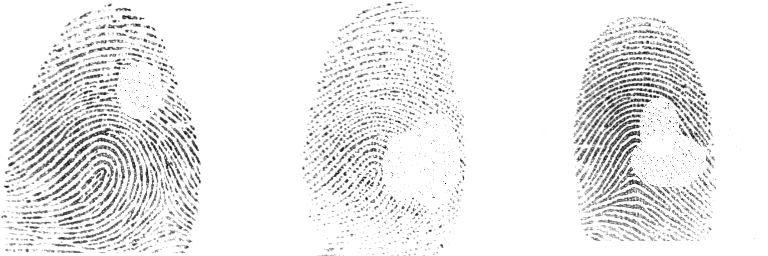
\includegraphics[scale=0.3]{figs/deterioration_1.png}}
\caption{Artificial fingerprint deterioration with holes}
\label{fig2}
\end{figure}

The second type of deterioration is oriented to simulate wet or dry fingers or noise or dirty scanning surfaces. This is achieved by summing a specific value to every pixel in the image until the mean of the image reaches 250. This removes some ridges and blurs the image. Finally, a gaussian noise is summed as it is showed in Fig.~\ref{fig3}.

\begin{figure}[htbp]
\centerline{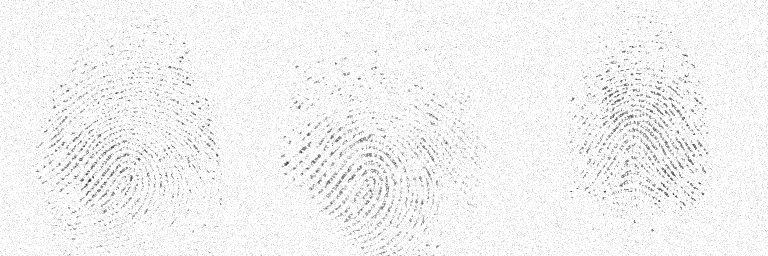
\includegraphics[scale=0.32]{figs/deterioration_2.png}}
\caption{Artificial fingerprint deterioration simulating finger or scanning modified conditions}
\label{fig3}
\end{figure}

Once the data is loaded and preprocessed, tuples are feeded into the model for making it to learn the optimum transformation that results in restored fingerprint images.

\section{Model Architecture}
\label{sec:MA}

Proposed architecture is composed by a generator that receives the image to enhance as input and returns the reconstructed image as output and a discriminator that determines whether or not an image was successfully reconstructed. Both convolutional structures will be detailed next.

Generator consists in a encoder and a decoder that configure an U-Net structure \cite{UNBIS}. The encoder is made up of eight sequentially connected convolutional layers, each one reducing the input height and width by a factor of two using same padding and strides of two. All layers use leakyrelu activation and batch normalization except for the first one. Similarly, decoder is made up of eight transpose convolutional layers, sometimes mistakenly called deconvolutional layers. In contrast to encoder, decoder layers increment by a factor of two height and width of input volumes which results in a final image of 256x256 pixels. All layers use batch normalization and relu activation and the first three layers use drop regularization. Fig.~\ref{fig4} shows a sketch of the generator and Table~\ref{tab1} of appendix specifies architecture details including number of filters on each layer.

\begin{figure}[htbp]
\centerline{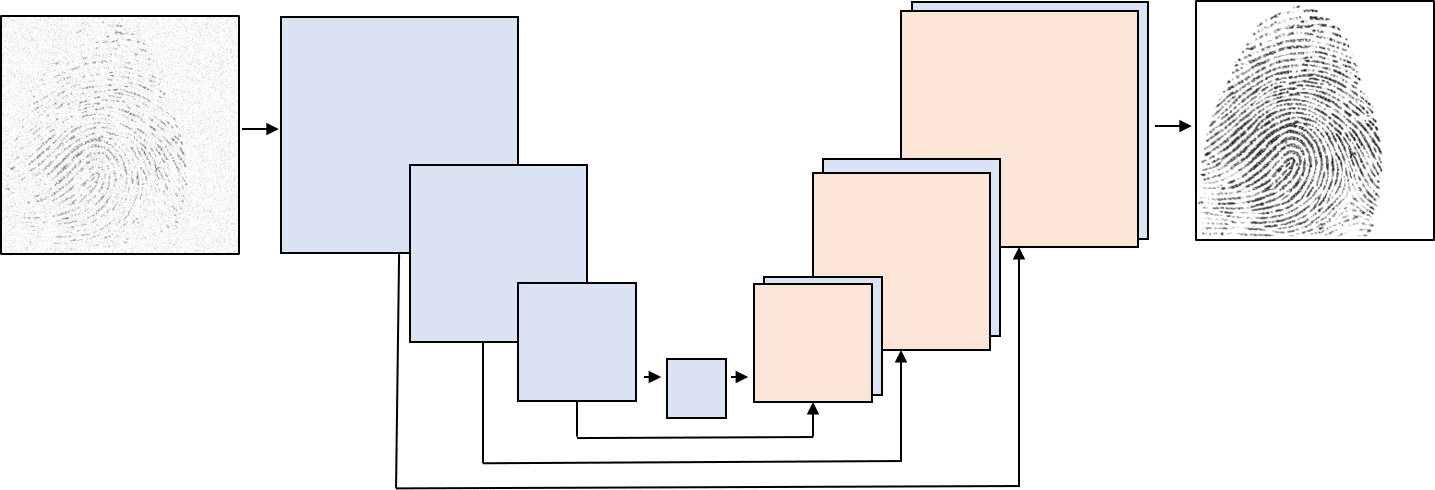
\includegraphics[scale=0.37]{figs/generator.png}}
\caption{Generator architecture}
\label{fig4}
\end{figure}

Discriminator is similar to a encoder since it applies convolutions to extract features from the input. However, unlike standard GANs, discriminator maps the input fingerprint to a 29x29 logits square rather than a scalar for deciding whether or not the image was correctly enhanced. Sigmoid function is applied to 29x29 output and then it is weighted to obtain the final value for the discriminator decision. This is called a PathGAN because each value of the 29x29 output, approximately corresponds to a 70x70 patch of the input image. Fig.~\ref{fig5} shows a sketch of the discriminator and Table~\ref{tab2} of appendix specifies architecture details including number of filters on each layer.

\begin{figure}[htbp]
\centerline{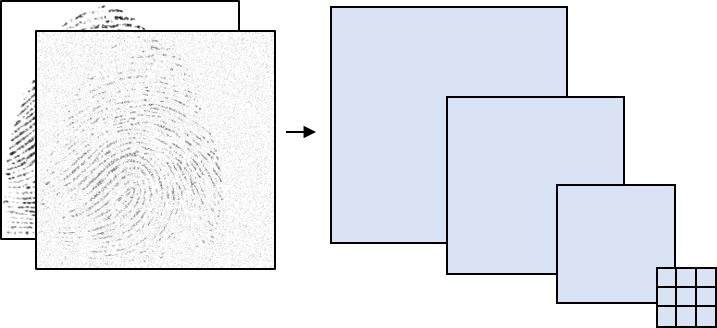
\includegraphics[scale=0.4]{figs/discriminator.png}}
\caption{Discriminator architecture}
\label{fig5}
\end{figure}

\section{Model training}
\label{sec:MT}

Let's recall that the main objective is make the generator to reconstruct and enhance deteriorate fingerprints the best way as possible. To achieve that, the model is trained through a optimization process that uses back propagation to calculate gradients and adam optimizer to update parameters. Since it is an adversarial architecture, there are two cost functions to minimize that will be described next.

The first cost function refers to the generator and it is made up of the sum of two terms. To obtain the first term, a deteriorated fingerprint of the dataset is passed through the generator. The reconstructed image is then compared to its ground truth using L1 norm. Second term is obtained concatenating reconstructed and deteriorated image, then passing the concatenation through the discriminator and finally calculating cross entropy with label equal to one meaning the intent of generator to fool the discriminator. Concatenation of deteriorated image gives to discriminator a context that helps to improve optimization process. Next equation summarizes what was previously described.
\begin{equation}
    Gen_{loss} = \alpha||y-gen(x)||_{[1]} - log(disc(x,gen(x)))
\end{equation}

Where $x$ corresponds to a deteriorated image, $gen(x)$ the reconstruction, $y$ the ground truth image, $disc(x,gen(x))$ the probability calculated passing the enhanced fingerprint through the discriminator and $\alpha$ defines the weight of reconstruction term.

The second cost function corresponds to counterpart of generator, the discriminator. It is also made up of the sum of two terms: the first is obtained concatenating reconstructed and deteriorated image, then passing the result through the discriminator and finally computing cross entropy with label equal to zero meaning the intent of discriminator of not being fooled by the generator. The second term is calculated similarly, however, it is concatenated the ground truth fingerprint instead of the reconstructed one and label is equal to one indicating that ground truth image is a real and correct reconstructed fingerprint.
\begin{equation}
    Disc_{loss} = -log(1-disc(x,gen(x)))-log(disc(x,y))
\end{equation}

Training process is configured as follows: tuples formed in the preprocessing step are grouped into batches of 48 elements. Adam optimizer is configured with $\beta_{1}=0.5$, $\beta_{2}=0.999$ and a learning rate of $0.00018$. In order to favour a correct reconstruction, $\alpha$ is set to 50. It was used a Nvidia Tesla K40 graphic card.

\section{Results}
\label{sec:R}

Fig.~\ref{fig6} shows three enhanced fingerprints using the proposed method and the first type of deterioration. It can be seen that the model was able to reconstruct the corrupted regions drawing the ridges that had been disappeared.

\begin{figure}[htbp]
\centerline{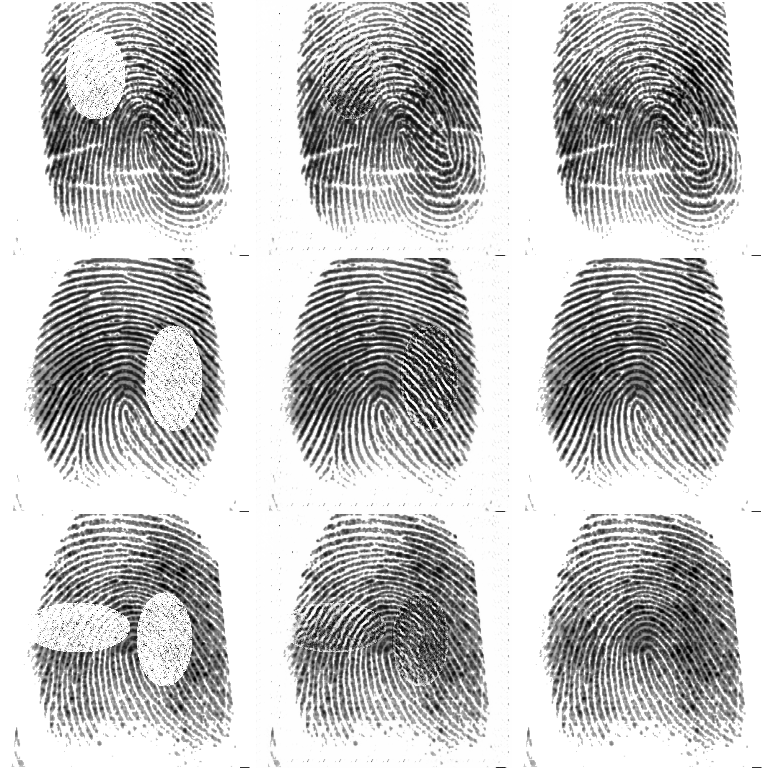
\includegraphics[scale=0.28]{figs/recons_1.png}}
\caption{Three successful reconstructions. First column is the deteriorated image, the second column is the enhanced fingerprint and the third column is the ground truth}
\label{fig6}
\end{figure}

The reconstruction of fingerprints altered with the second type of deterioration is shown in Fig.~\ref{fig7}. The most of the ridges were recovered and the noise was diminished improving fingerprint clarity and quality.

\begin{figure}[htbp]
\centerline{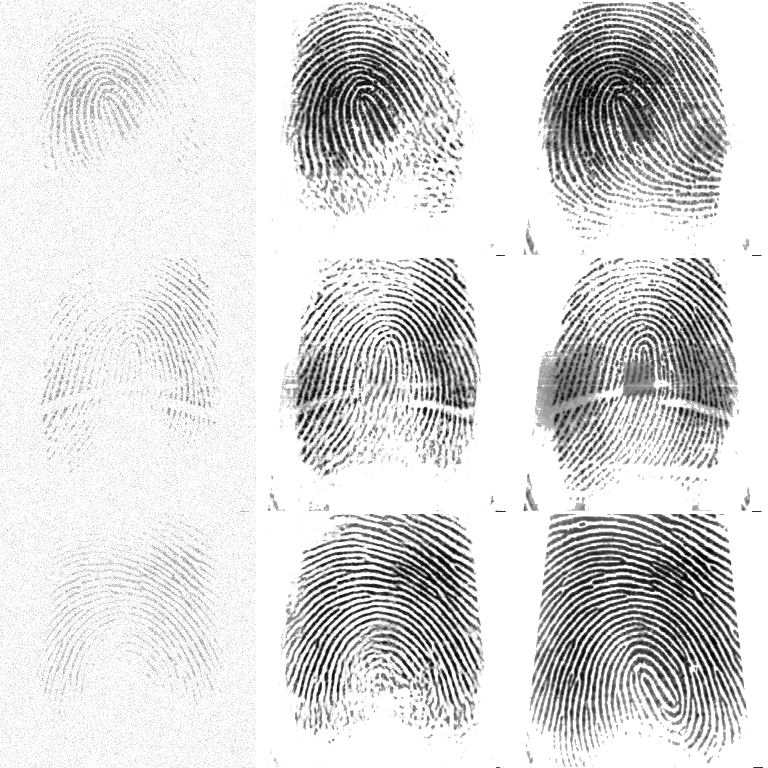
\includegraphics[scale=0.28]{figs/recons_2.png}}
\caption{Three successful enhancements. First column is the deteriorated image, the second column is the enhanced fingerprint and the third column is the ground truth}
\label{fig7}
\end{figure}

In contrast to showed results, there were some fingerprint examples that could not be restored effectively as shown in Fig.~\ref{fig8}. In some cases the deterioration caused a high level of corruption in the fingerprints, so, it was almost impossible to achieve a successful enhancement. On the other hand, fingerprints itself had noisy structures and saturated ridges that got over the algorithm capacity.

\begin{figure}[htbp]
\centerline{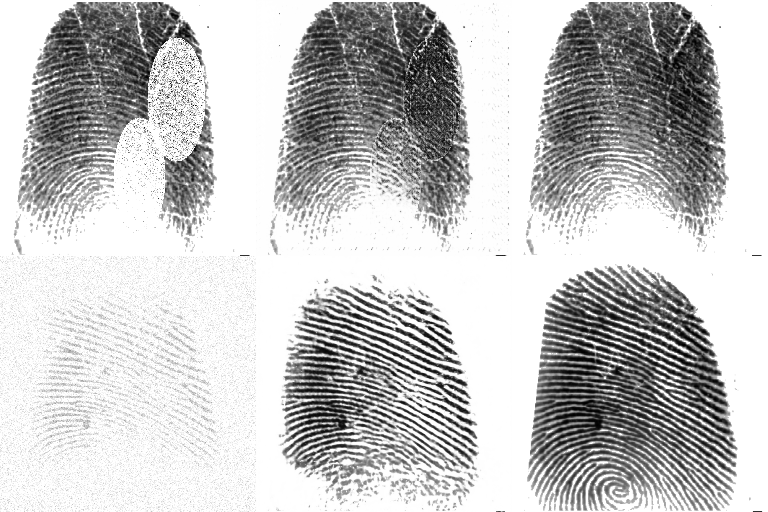
\includegraphics[scale=0.28]{figs/recons_failed.png}}
\caption{Two failed examples. First column is the deteriorated image, the second column is the enhanced fingerprint and the third column is the ground truth}
\label{fig8}
\end{figure}

The first test was carried out using the Receiver Operating Characteristic (ROC), a well-accepted measure to express performance of 1:1 matchers \cite{RROCCMC}. Matching scores were computed between images to reconstruct and the ground truth images and between reconstructed images and ground truth images. These scores are compared to a threshold to determine whether or not the pair belongs to the same person. Finally, CMC curve is obtained plotting the True Positive Rate (TPR) and False Positive Rate (FPR) for different thresholds as can be seen in Fig.~\ref{fig9}.

\begin{figure}[htbp]
\centerline{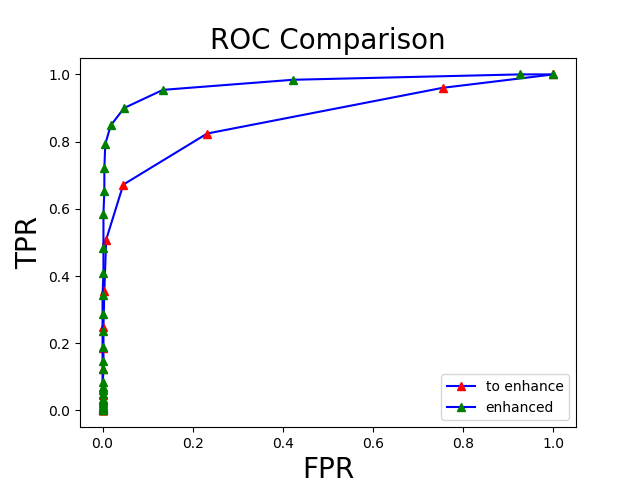
\includegraphics[scale=0.45]{figs/roc_comparison.png}}
\caption{ROC curve comparison before and after reconstruction}
\label{fig9}
\end{figure}

Since TPR stays at vertical axis and FPR at horizontal axis, the more upper left the points are in the graph, the better the model performance. The enhanced fingerprints curve lies at the top left side of the graph while the deteriorated fingerprints curve is located at a more lower right position. Additionally, the Area Under the Curve (AUC) augmented from 0.85 to 0.92 which means that the enhancer model improved the accuracy of the matching process.

The Cumulative Match Curve (CMC) is used in the second prove. Since it is a 1:m matching algorithm tester, the matching score must be computed on every possible tuple formed by a deteriorated image and a ground truth image and a enhanced image and a ground truth image. The curves are obtained following steps described in \cite{RROCCMC} and results are showed in Fig.~\ref{fig10}.

\begin{figure}[htbp]
\centerline{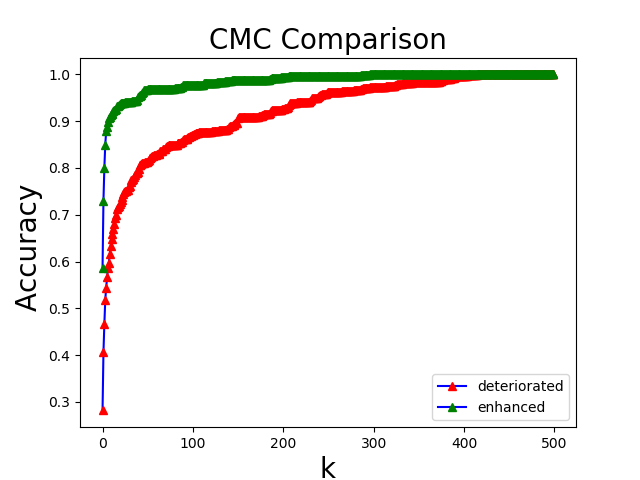
\includegraphics[scale=0.45]{figs/cmc_comparison.png}}
\caption{CMC curve comparison before and after reconstruction}
\label{fig10}
\end{figure}

CMC curve shows the cumulative probability of obtaining a correct match based on computed scores within the first $k$ highest matching scores. In contrast to deteriorated images curve, enhanced fingerprints curve presents a higher value at $k$ equal to one and a steeper slope at that point. This indicates a better performance while implementing a 1:m fingerprint identification algorithm through sorting \cite{RROCCMC}.

The final performance metric consists on measuring average fingerprint image quality of the validation dataset before and after reconstruction. The nfiq measure scores a high quality fingerprint with a value of 1 and a low quality fingerprint with a value of 5. Fig.~\ref{fig11} shows that average quality of images improved after enhancement. The difference of fingerprint quality with respect to ground truth images decreased from 70\% to 18\%.

\begin{figure}[htbp]
\centerline{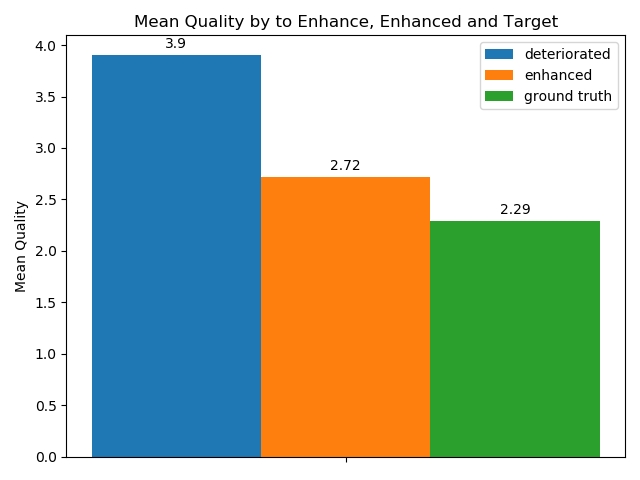
\includegraphics[scale=0.4]{figs/mean_qualities.png}}
\caption{Quality mean curve comparison before and after reconstruction}
\label{fig11}
\end{figure}

\section{Conclusion}
\label{sec:CON}

The generative model showed a good performance on the fingerprint reconstruction task. Both ROC and CMC curves demonstrated an improvement of matching accuracy after the enhancement process. In addition, average fingerprint quality measured with nfiq algorithm increased. However, it is worth mentioning that if the fingerprints are highly corrupted or deteriorated the model will not be not able to make a successful reconstruction. This is because filters used in convolutions need a minimum of information to extract features and represent them correctly in the output image.


\section{Future work}
\label{sec:FW}

More complex deterioration algorithms can be studied in order to simulate real world scenarios. Additionally, in order to improve algorithm generalization and performance it can be developed a dataset containing real fingerprint corruptions and its corresponding ground truths. On the other hand, a dataset can be built with fingerprints and its corresponding binarization, a crucial component of the minutiae extraction process.

\printcredits

%% Loading bibliography style file
%\bibliographystyle{model1-num-names}
\bibliographystyle{cas-model2-names}

% Loading bibliography database
\bibliography{cas-refs}

%\vskip3pt

\bio{figs/foto_cristian.png}
\textbf{Cristian Yesid Andrade Hernández} courses ninth semester of Electronic Engineering at Universidad de los Andes. Interested in technology applications that involves machine learning, pattern recognition, robotics, control and artificial intelligence. Algorithms and programming skills cover Java, C\#, Python, JavaScript, C++, Visual Basic and Matlab. Two years of experience teaching programming as tutor in a engineering course at university. Internship at Colpatria Group Company: Olimpia IT working on automatic testing of the software.
\endbio

\onecolumn
\appendix
\section{My Appendix}

\begin{table}[htbp]
\caption{Architecture details of generator}
\begin{tabular}{|c|c|c|c|c|c|c|c|c|}
\hline
{\color[HTML]{000000} \textbf{Layer}} &
  {\color[HTML]{000000} \textbf{Strides}} &
  {\color[HTML]{000000} \textbf{Padding}} &
  {\color[HTML]{000000} \textbf{Filters}} &
  {\color[HTML]{000000} \textbf{Input size}} &
  {\color[HTML]{000000} \textbf{Output size}} &
  {\color[HTML]{000000} \textbf{Batchnorm}} &
  {\color[HTML]{000000} \textbf{Activation}} &
  {\color[HTML]{000000} \textbf{Dropout}} \\ \hline
{\color[HTML]{000000} Conv1} &
  {\color[HTML]{000000} (4,4)} &
  {\color[HTML]{000000} same} &
  {\color[HTML]{000000} 64} &
  {\color[HTML]{000000} (256,256,1)} &
  {\color[HTML]{000000} (128,128,64)} &
  {\color[HTML]{000000} No} &
  {\color[HTML]{000000} LeakyRelu} &
  {\color[HTML]{000000} No} \\ \hline
{\color[HTML]{000000} Conv2} &
  {\color[HTML]{000000} (4,4)} &
  {\color[HTML]{000000} same} &
  {\color[HTML]{000000} 128} &
  {\color[HTML]{000000} (128,128,64)} &
  {\color[HTML]{000000} (64,64,128)} &
  {\color[HTML]{000000} Yes} &
  {\color[HTML]{000000} LeakyRelu} &
  {\color[HTML]{000000} No} \\ \hline
{\color[HTML]{000000} Conv3} &
  {\color[HTML]{000000} (4,4)} &
  {\color[HTML]{000000} same} &
  {\color[HTML]{000000} 256} &
  {\color[HTML]{000000} (64,64,128)} &
  {\color[HTML]{000000} (32,32,256)} &
  {\color[HTML]{000000} Yes} &
  {\color[HTML]{000000} LeakyRelu} &
  {\color[HTML]{000000} No} \\ \hline
{\color[HTML]{000000} Conv4} &
  {\color[HTML]{000000} (4,4)} &
  {\color[HTML]{000000} same} &
  {\color[HTML]{000000} 512} &
  {\color[HTML]{000000} (32,32,256)} &
  {\color[HTML]{000000} (16,16,512)} &
  {\color[HTML]{000000} Yes} &
  {\color[HTML]{000000} LeakyRelu} &
  {\color[HTML]{000000} No} \\ \hline
{\color[HTML]{000000} Conv5} &
  {\color[HTML]{000000} (4,4)} &
  {\color[HTML]{000000} same} &
  {\color[HTML]{000000} 512} &
  {\color[HTML]{000000} (16,16,512)} &
  {\color[HTML]{000000} (8,8,512)} &
  {\color[HTML]{000000} Yes} &
  {\color[HTML]{000000} LeakyRelu} &
  {\color[HTML]{000000} No} \\ \hline
{\color[HTML]{000000} Conv6} &
  {\color[HTML]{000000} (4,4)} &
  {\color[HTML]{000000} same} &
  {\color[HTML]{000000} 512} &
  {\color[HTML]{000000} (8,8,512)} &
  {\color[HTML]{000000} (4,4,512)} &
  {\color[HTML]{000000} Yes} &
  {\color[HTML]{000000} LeakyRelu} &
  {\color[HTML]{000000} No} \\ \hline
{\color[HTML]{000000} Conv7} &
  {\color[HTML]{000000} (4,4)} &
  {\color[HTML]{000000} same} &
  {\color[HTML]{000000} 512} &
  {\color[HTML]{000000} (4,4,512)} &
  {\color[HTML]{000000} (2,2,512)} &
  {\color[HTML]{000000} Yes} &
  {\color[HTML]{000000} LeakyRelu} &
  {\color[HTML]{000000} No} \\ \hline
{\color[HTML]{000000} Conv8} &
  {\color[HTML]{000000} (4,4)} &
  {\color[HTML]{000000} same} &
  {\color[HTML]{000000} 512} &
  {\color[HTML]{000000} (2,2,512)} &
  {\color[HTML]{000000} (1,1,512)} &
  {\color[HTML]{000000} Yes} &
  {\color[HTML]{000000} LeakyRelu} &
  {\color[HTML]{000000} No} \\ \hline
{\color[HTML]{000000} TransConv1} &
  {\color[HTML]{000000} (4,4)} &
  {\color[HTML]{000000} same} &
  {\color[HTML]{000000} 512} &
  {\color[HTML]{000000} (1,1,512)} &
  {\color[HTML]{000000} (2,2,512)} &
  {\color[HTML]{000000} Yes} &
  {\color[HTML]{000000} Relu} &
  {\color[HTML]{000000} Yes} \\ \hline
{\color[HTML]{000000} TransConv2} &
  {\color[HTML]{000000} (4,4)} &
  {\color[HTML]{000000} same} &
  {\color[HTML]{000000} 512} &
  {\color[HTML]{000000} (2,2,512)} &
  {\color[HTML]{000000} (4,4,512)} &
  {\color[HTML]{000000} Yes} &
  {\color[HTML]{000000} Relu} &
  {\color[HTML]{000000} Yes} \\ \hline
{\color[HTML]{000000} TransConv3} &
  {\color[HTML]{000000} (4,4)} &
  {\color[HTML]{000000} same} &
  {\color[HTML]{000000} 512} &
  {\color[HTML]{000000} (4,4,512)} &
  {\color[HTML]{000000} (8,8,512)} &
  {\color[HTML]{000000} Yes} &
  {\color[HTML]{000000} Relu} &
  {\color[HTML]{000000} Yes} \\ \hline
{\color[HTML]{000000} TransConv4} &
  {\color[HTML]{000000} (4,4)} &
  {\color[HTML]{000000} same} &
  {\color[HTML]{000000} 512} &
  {\color[HTML]{000000} (8,8,512)} &
  {\color[HTML]{000000} (16,16,512)} &
  {\color[HTML]{000000} Yes} &
  {\color[HTML]{000000} Relu} &
  {\color[HTML]{000000} No} \\ \hline
{\color[HTML]{000000} TransConv5} &
  {\color[HTML]{000000} (4,4)} &
  {\color[HTML]{000000} same} &
  {\color[HTML]{000000} 256} &
  {\color[HTML]{000000} (16,16,512)} &
  {\color[HTML]{000000} (32,32,256)} &
  {\color[HTML]{000000} Yes} &
  {\color[HTML]{000000} Relu} &
  {\color[HTML]{000000} No} \\ \hline
{\color[HTML]{000000} TransConv6} &
  {\color[HTML]{000000} (4,4)} &
  {\color[HTML]{000000} same} &
  {\color[HTML]{000000} 128} &
  {\color[HTML]{000000} (32,32,256)} &
  {\color[HTML]{000000} (64,64,128)} &
  {\color[HTML]{000000} Yes} &
  {\color[HTML]{000000} Relu} &
  {\color[HTML]{000000} No} \\ \hline
{\color[HTML]{000000} TransConv7} &
  {\color[HTML]{000000} (4,4)} &
  {\color[HTML]{000000} same} &
  {\color[HTML]{000000} 64} &
  {\color[HTML]{000000} (64,64,128)} &
  {\color[HTML]{000000} (128,128,64)} &
  {\color[HTML]{000000} Yes} &
  {\color[HTML]{000000} Relu} &
  {\color[HTML]{000000} No} \\ \hline
{\color[HTML]{000000} TransConv8} &
  {\color[HTML]{000000} (4,4)} &
  {\color[HTML]{000000} same} &
  {\color[HTML]{000000} 1} &
  {\color[HTML]{000000} (128,128,64)} &
  {\color[HTML]{000000} (256,256,1)} &
  {\color[HTML]{000000} Yes} &
  {\color[HTML]{000000} Tanh} &
  {\color[HTML]{000000} No} \\ \hline
\end{tabular}
\label{tab1}
\end{table}

\begin{table}[htbp]
\caption{Architecture details of discriminator}
\begin{tabular}{|c|c|c|c|c|c|c|c|c|}
\hline
{\color[HTML]{000000} \textbf{Layer}} &
  {\color[HTML]{000000} \textbf{Strides}} &
  {\color[HTML]{000000} \textbf{Padding}} &
  {\color[HTML]{000000} \textbf{Filters}} &
  {\color[HTML]{000000} \textbf{Input size}} &
  {\color[HTML]{000000} \textbf{Output size}} &
  {\color[HTML]{000000} \textbf{Batchnorm}} &
  {\color[HTML]{000000} \textbf{Activation}} &
  {\color[HTML]{000000} \textbf{Dropout}} \\ \hline
{\color[HTML]{000000} Conv1} &
  {\color[HTML]{000000} (4,4)} &
  {\color[HTML]{000000} same} &
  {\color[HTML]{000000} 64} &
  {\color[HTML]{000000} (256,256,1)} &
  {\color[HTML]{000000} (128,128,64)} &
  {\color[HTML]{000000} Yes} &
  {\color[HTML]{000000} LeakyRelu} &
  {\color[HTML]{000000} No} \\ \hline
{\color[HTML]{000000} Conv2} &
  {\color[HTML]{000000} (4,4)} &
  {\color[HTML]{000000} same} &
  {\color[HTML]{000000} 128} &
  {\color[HTML]{000000} (128,128,64)} &
  {\color[HTML]{000000} (64,64,128)} &
  {\color[HTML]{000000} Yes} &
  {\color[HTML]{000000} LeakyRelu} &
  {\color[HTML]{000000} No} \\ \hline
{\color[HTML]{000000} Conv3} &
  {\color[HTML]{000000} (4,4)} &
  {\color[HTML]{000000} same} &
  {\color[HTML]{000000} 256} &
  {\color[HTML]{000000} (64,64,128)} &
  {\color[HTML]{000000} (32,32,256)} &
  {\color[HTML]{000000} Yes} &
  {\color[HTML]{000000} LeakyRelu} &
  {\color[HTML]{000000} No} \\ \hline
{\color[HTML]{000000} Con4} &
  {\color[HTML]{000000} (1,1)} &
  {\color[HTML]{000000} same} &
  {\color[HTML]{000000} 512} &
  {\color[HTML]{000000} (32,32,256)} &
  {\color[HTML]{000000} (32,32,512)} &
  {\color[HTML]{000000} Yes} &
  {\color[HTML]{000000} LeakyRelu} &
  {\color[HTML]{000000} No} \\ \hline
{\color[HTML]{000000} Conv5} &
  {\color[HTML]{000000} (1,1)} &
  {\color[HTML]{000000} same} &
  {\color[HTML]{000000} 1} &
  {\color[HTML]{000000} (32,32,512)} &
  {\color[HTML]{000000} (29,29,1)} &
  {\color[HTML]{000000} No} &
  {\color[HTML]{000000} None} &
  {\color[HTML]{000000} No} \\ \hline
\end{tabular}
\label{tab2}
\end{table}

\end{document}